\documentclass[reqno,12pt]{amsart}

\usepackage[colorlinks=true]{hyperref}
\hypersetup{urlcolor=blue, citecolor=red}

\usepackage{amssymb,graphicx,color}
\usepackage[latin1]{inputenc}

\usepackage[capitalize,nameinlink,noabbrev]{cleveref}

%The Layout
\setlength{\oddsidemargin}{0pt}
\setlength{\evensidemargin}{0pt}
\setlength{\textheight}{42\baselineskip}
\setlength{\textwidth}{6in}
%\addtolength{\headheight}{0.7in}

\theoremstyle{plain}% default
\newtheorem{thm}{Theorem}[section]
\newtheorem{lem}{Lemma}[section]
\newtheorem{prop}{Proposition}[section]
\newtheorem{cor}{Corollary}[section]
\newtheorem{defs}{Definition}[section]
\newtheorem{prob}{Problem}[section]
\newtheorem{stdhyp}{Hypothesis}[section]
\theoremstyle{definition}
\newtheorem{rmk}{Remark}[section]
\newtheorem{fact}{Fact}[section]

\newcommand{\NN}{{\mathbb{N}}}
\newcommand{\ZZ}{{\mathbb{Z}}}
\newcommand{\RR}{{\mathbb{R}}}
\newcommand{\CC}{{\mathbb{C}}}
\newcommand{\QQ}{{\mathbb{Q}}}
\newcommand{\bfu}{\mathbf{u}}
\newcommand{\bfv}{\mathbf{v}}
\newcommand{\bfw}{\mathbf{w}}
\newcommand{\bfe}{\mathbf{e}}
\newcommand{\bfa}{\mathbf{a}}
\newcommand{\bfb}{\mathbf{b}}
\newcommand{\bfg}{\mathbf{g}}
\newcommand{\bff}{\mathbf{f}}
\newcommand{\bfh}{\mathbf{h}}
\newcommand{\bfq}{\mathbf{q}}
\newcommand{\bfx}{\mathbf{x}}
\newcommand{\bfy}{\mathbf{y}}
\newcommand{\bfz}{\mathbf{z}}
\newcommand{\bfr}{\mathbf{r}}
\newcommand{\bfn}{\mathbf{n}}
\newcommand{\bfA}{\mathbf{A}}
\newcommand{\bfB}{\mathbf{B}}
\newcommand{\bfD}{\mathbf{D}}
\newcommand{\bfE}{\mathbf{E}}
\newcommand{\bfI}{\mathbf{I}}
\newcommand{\bfU}{\mathbf{U}}
\newcommand{\bfF}{\mathbf{F}}
\newcommand{\bfR}{\mathbf{R}}
\newcommand{\bfX}{\mathbf{X}}
\newcommand{\bfk}{\mathbf{k}}
\newcommand{\bfj}{\mathbf{j}}
\newcommand{\bfl}{\mathbf{l}}
\newcommand{\bfell}{\boldsymbol{\ell}}
\newcommand{\bfL}{\mathbf{L}}
\newcommand{\bfT}{\mathbf{T}}
\newcommand{\bfM}{\mathbf{M}}
\newcommand{\bfzero}{\mathbf{0}}
\newcommand{\fke}{\mathfrak{e}}
\newcommand{\fkE}{\mathfrak{E}}
\newcommand{\fkf}{\mathfrak{f}}
\newcommand{\fkF}{\mathfrak{F}}
\newcommand{\fkg}{\mathfrak{g}}
\newcommand{\fkG}{\mathfrak{G}}
\newcommand{\fkh}{\mathfrak{h}}
\newcommand{\fkH}{\mathfrak{H}}
\newcommand{\bfcurl}{\mbox{\bf curl}\;}
\newcommand{\bfalpha}{{\boldsymbol{\alpha}}}
\newcommand{\bfvarphi}{\boldsymbol{\varphi}}
\newcommand{\bfPhi}{\boldsymbol{\Phi}}
\newcommand{\bfpsi}{\boldsymbol{\psi}}
\newcommand{\bfxi}{\boldsymbol{\xi}}
\newcommand{\bfnabla}{\boldsymbol{\nabla}}
\newcommand{\bfdelta}{\boldsymbol{\delta}}
\newcommand{\bfomega}{\boldsymbol{\omega}}
\newcommand{\bfsigma}{\boldsymbol{\sigma}}
\newcommand{\bftau}{\boldsymbol{\tau}}
\newcommand{\bfeta}{\boldsymbol{\eta}}
\newcommand{\bfzeta}{\boldsymbol{\zeta}}
\newcommand{\bfkappa}{\boldsymbol{\kappa}}
\newcommand{\bfvarrho}{\boldsymbol{\varrho}}
\newcommand{\bfchi}{\boldsymbol{\chi}}
\newcommand{\define}{\stackrel{\mathrm{def}}{=}}
\newcommand{\Ccal}{{\mathcal C}}
\newcommand{\Acal}{{\mathcal A}}
\newcommand{\Bcal}{{\mathcal B}}
\newcommand{\Fcal}{{\mathcal F}}
\newcommand{\Scal}{{\mathcal S}}
\newcommand{\Ncal}{{\mathcal N}}
\newcommand{\Rcal}{{\mathcal R}}
\newcommand{\Qcal}{{\mathcal Q}}
\newcommand{\Gcal}{{\mathcal G}}
\newcommand{\Kcal}{{\mathcal K}}
\newcommand{\Xcal}{{\mathcal X}}
\newcommand{\Ycal}{{\mathcal Y}}
\newcommand{\Zcal}{{\mathcal Z}}
\newcommand{\Vcal}{{\mathcal V}}
\newcommand{\Wcal}{{\mathcal W}}
\newcommand{\per}{{\mathrm{per}}}
\newcommand{\ch}{{\mathrm{ch}}}
\newcommand{\loc}{{\mathrm{loc}}}
\newcommand{\zave}[1]{\dot{#1}}
\newcommand{\Ecal}{{\mathcal E}}
\newcommand{\Mcal}{{\mathcal M}}
\newcommand{\Pcal}{{\mathcal P}}
\newcommand{\Dcal}{{\mathcal D}}
\newcommand{\Tcal}{{\mathcal T}}
\newcommand{\Ucal}{{\mathcal U}}
\newcommand{\Lcal}{{\mathcal L}}
\newcommand{\Ocal}{{\mathcal O}}
\newcommand{\Gr}{\mathrm{G}}
\newcommand{\Rey}{\mathrm{Re}}
\newcommand{\rmD}{\mathrm{D}}
\newcommand{\rmH}{\mathrm{H}}
\newcommand{\rmP}{\mathrm{P}}
\newcommand{\rmS}{\mathrm{S}}
\newcommand{\rmKo}{\mathrm{Ko}}
\newcommand{\rmKr}{\mathrm{Kr}}
\newcommand{\rmd}{\mathrm{d}}
\newcommand{\rmw}{\mathrm{w}}
\newcommand{\rmv}{\mathrm{v}}
\newcommand{\rmreg}{\mathrm{reg}}
\newcommand{\rmb}{\mathrm{b}}
\newcommand{\rmg}{\mathrm{g}}
\newcommand{\rmc}{\mathrm{c}}
\newcommand{\rmr}{\mathrm{r}}
\newcommand{\rms}{\mathrm{s}}
\newcommand{\sfA}{\mathsf{A}}
\newcommand{\sfD}{\mathsf{D}}
\newcommand{\sfT}{\mathsf{T}}
\newcommand{\sfI}{\mathsf{I}}
\newcommand{\sfJ}{\mathsf{J}}
\newcommand{\sfS}{\mathsf{S}}
\newcommand{\sfsigma}{\mathsf{\sigma}}
\newcommand{\sftau}{\mathsf{\tau}}
\newcommand{\sgn}{\operatorname{sgn}}
\newcommand{\Id}{\operatorname{Id}}
\newcommand{\tr}{{\operatorname{tr}}}
\newcommand{\supp}{\operatorname*{supp}}
\newcommand{\Tr}{\operatorname{Tr}}
\newcommand{\Cyl}{\operatorname{\mathcal{C}_{yl}}}
\newcommand{\Syl}{\operatorname{\mathcal{S}_{yl}}}
\newcommand{\nse}{{\operatorname{nse}}}
\newcommand{\cyl}{{\operatorname{cyl}}}
\newcommand{\sss}{{\operatorname{sss}}}
\newcommand{\fpsss}{{\operatorname{fpsss}}}
\newcommand{\wsss}{{\operatorname{wsss}}}
\newcommand{\tasss}{{\operatorname{tasss}}}
\newcommand{\inv}{{\operatorname{inv}}}
\newcommand{\Linv}{{\operatorname{L-inv}}}
\newcommand{\Einv}{{\operatorname{E-inv}}}
\newcommand{\sinv}{{\operatorname{\sigma-inv}}}
\newcommand{\Piinv}{{\operatorname{\Pi-inv}}}
\newcommand{\average}[1]{\langle{#1}\rangle}
\newcommand{\dual}[1]{\langle{#1}\rangle}
\newcommand{\inner}[1]{({#1})}
\newcommand{\dinner}[1]{(\!({#1})\!)}
\newcommand{\Lim}{\operatorname*{\textsc{Lim}}_{T\rightarrow \infty}}
\newcommand{\co}{\operatorname*{\text{co}}}
\newcommand{\paratitle}[1]{\vspace{\baselineskip} \noindent \emph{{#1}}}
%\newcommand{\comment}[1]{\textcolor{red}{\framebox{\parbox{0.9\textwidth}{\textbf{#1}}}}}
\newcommand{\comment}[1]{\textcolor{red}{\textbf{#1}}}
\newcommand{\doshow}[1]{#1}
\newcommand{\dontshow}[1]{}
\newcommand{\extra}[1]{\dontshow{#1}} % use \show to show the extra stuff or \donotshow not to show it

%\mathchardef\mhyphen="2D

\renewcommand{\subjclassname}{$2020$ Mathematics Subject Classification}

\renewcommand{\theenumi}{\roman{enumi}}

\begin{document}
\numberwithin{equation}{section}

% Article info

\title[Strong order 1 convergence of Euler-Maruyama for Random ODEs]{Conditions for the strong order 1 convergence of the Euler-Maruyama approximation for Random Ordinary Differential Equations}

\author[R. M. S. Rosa]{Ricardo M. S. Rosa}

\author[P. E. Kloeden]{Peter E. Kloeden}

\address[Ricardo M. S. Rosa]{Instituto de Matem\'atica, Universidade Federal do Rio de Janeiro, Brazil}
\address[Peter E. Kloeden]{Mathematics Department, University of Tubingen, Germany}

\email[R. M. S. Rosa]{rrosa@im.ufrj.br}
\email[P. E. Kloeden]{kloeden@math.uni-frankfurt.de}

\date{\today}

%\thanks{This work was partly supported by the CNPq, Bras\'{\i}lia, Brazil and by the NSF grant ???.}

\subjclass[2000]{76D05, 76D06, 35Q30, 37L99}
\keywords{random ordinary differential equations, Euler-Maruyama method, strong convergence, It\^o process, point process}.

\begin{abstract}
It is well known that the Euler-Maruyama method of approximating a random ordinary differential equation $\mathrm{d}X_t/\mathrm{d}t = f(t, X_t, Y_t)$ driven by a stochastic process $\{Y_t\}_t$ with $\theta$-H\"older sample paths is estimated to be of strong order $\theta$ with respect to the time step, provided $f=f(t, x, w)$ is sufficiently regular. Here, we show that, in common situations, it is possible to exploit ``hidden'' conditions on the noise and prove that the strong convergence is actually of order 1, regardless of much regularity on the sample paths. This applies to It\^o process noises (such as Wiener, Ornstein-Uhlenbeck, and Geometric Brownian process), which are H\"older continuous, and to point processes (such as Poisson point processes and Hawkes self-exciting processes), which are not even continuous and have jump-type discontinuities, as well as to transport processes. The order 1 convergence follows from not estimating directly the local error, but, instead, adding up the local steps and estimating the compound error. In the case of an It\^o noise, the compound error is then estimated via It\^o formula and the It\^o isometry. In the case of a point process or a transport process, a monotonic bound is exploited. We HOPEFULLY complement the result by giving examples where some of the conditions are not met and the order of convergence seems indeed to be less than 1.
\end{abstract}

\maketitle

\section{Introduction}

Consider the following initial value problem for a \textbf{random ordinary differential equation (RODE)}:
\begin{equation}
  \label{rodeeq}
  \begin{cases}
    \displaystyle \frac{\mathrm{d}X_t}{\mathrm{d} t} = f(t, X_t, Y_t), \qquad 0 \leq t \leq T, \\
    \left. X_t \right|_{t = 0} = X_0,
  \end{cases}
\end{equation}
on a time interval $I=[0, T]$, with $T > 0$, and where the noise $\{Y_t\}_{t\in I}$ is a given stochastic process. The sample space is denoted by $\Omega$.

The Euler-Maruyama method for solving this initial value problem consists in approximating the solution on a uniform time mesh $t_j = j\Delta t_N$, $j = 0, \ldots, N$, with fixed time step $\Delta t_N = T/N$, for a given $N\in \mathbb{N}$. In such a mesh, the Euler-Maruyama scheme takes the form
\begin{equation}
  \label{emscheme}
  X_{t_j}^N = X_{t_{j-1}}^N + \Delta t_N f(t_{j-1}, X_{t_{j-1}}^N, Y_{t_{j-1}}), \qquad j = 1, \ldots, N,
\end{equation}
with the initial condition
\begin{equation}
  \label{iccondition}
  X_0^N = X_0.
\end{equation}
Notice $t_j = j\Delta t_N = jT/N$ also depends on $N$, but we do not make this dependency explicit, for the sake of notational simplicity.

When the noise $\{Y_t\}_{t\in I}$ has $\theta$-H\"older continuous sample paths, it can be show \cite{GruneKloeden2001}, under further suitable conditions, that the Euler-Maruyama scheme converges strongly with order $\theta$ with the time step, i.e. there exists a constant $C \geq 0$ such that
\begin{equation}
    \label{strongordertheta}
    \max_{j=0, \ldots, N}\mathbb{E}\left[ \left| X_{t_j} - X_{t_j}^N \right| \right] \leq C \Delta t_N^\theta, \qquad \forall N \in \mathbb{N},
\end{equation}
where $\mathbb{E}[\cdot]$ indicates the expectation of a random variable on $\Omega$.

Our aim is to show that, in many classical examples, it is possible to exploit further conditions that yield in fact a strong order 1 convergence, with the sample paths still being H\"older continuous or even have jump discontinuities. This is the case, for instance, when the noise is an It\^o noise, or when the equation is semi-separable and the noise is a point process or a transport process.

Indeed, many common H\"older functions are actually of bounded variation, such as $t\mapsto t^{1/3}$ and $t\mapsto \sin(\omega t)^{1/5}$. This is a common situation when the noise is a transport process $Y_t = g(t, Y_0)$, for a random vector $Y_0 = Y_0(\omega)$. Even functions with jump discontinuities, such as those in point-processes, are of bounded variation. Being of bounded variation, it is possible to control their steps and obtain the strong order 1 convergence.

In the case of an It\^o noise, the sample paths are typically H\"older continuous with exponent 1/2 and are not of bounded variation. In this case, however, the It\^o isometry reveals futher regularity that can be used to yield a strong order 1 convergence.

More precisely, for the semi-separable case, we assume $f$ is of the form 
\[
    f(t, x, y) = a(t, y)h(x) + b(t, y).  
\]
In this case, we assume the processes $\{a(t, Y_t)\}_{t\in I}$ and $\{b(t, Y_t)\}_{t\in I}$ have their steps bounded by a monotonic process, which typically happens for point processes, i.e.
\[
|a(t+\tau, Y_{t+\tau}) - a(t, Y_t)| \leq A_t, \quad |b(t+\tau, Y_{t+\tau}) - b(t, Y_t)| \leq B_t,
\]
where $\{A_t\}_{t\in I}$ and $\{B_t\}_{t\in I}$ have monotonically non-decreasing sample paths. Under further suitable conditions (see \cref{thmsemiseparablemonotonicbound}), we show that the Euler-Maruyama method is of strong order 1, i.e. \eqref{strongordertheta} holds with $\theta=1$.

Even if the structure of the equation is not exactly semi-separable but it is somehow possible to bound the steps $|f(t+\tau, X_t, Y_{t+\tau}) - a(t, X_t, Y_t)|$ by a suitable process with monotonic non-decreasing sample paths, it is possible to prove the strong order 1 convergence (see \cref{thmmonotonicbound}).

For the It\^o noise case, we consider a general equation of the form \eqref{rodeeq}, with a noise defined as an \textbf{It\^o process} $\{Y_t\}_{t\geq 0}$, satisfying
\begin{equation}
  \mathrm{d}Y_t = A_t \;\mathrm{d}t + B_t \;\mathrm{d}W_t,
\end{equation}
We are not solving for $Y_t$, nor approximating it numerically, otherwise we would actually need to consider a system of stochastic differential equations. Instead, we assume it is a known process that can be computed analytically, such as a Wiener process, an Ornstein-Uhlenbeck process, or a geometric Brownian motion. With those in mind, $A_t$ and $B_t$ may be originally given in terms of $\{W_t\}_{t\geq 0}$ and $\{Y_t\}_{t\in I}$, but the general assumption is only given in terms of $\{A_t\}_{t\in I}$ and $\{B_t\}_{t\in I}$.

In the case that $f=f(t, x, y)$ is twice continuously differentiable, the It\^o formula applies and we show, under suitable conditions on $\{A_t\}_{t\in I}$, $\{B_t\}_{t\in I}$ and the derivatives of $f$, that the Euler-Maruyama method is of strong order 1, i.e. \eqref{strongordertheta} holds with $\theta=1$.

In order to make the main idea clear cut, here are the options we have for estimating the error:
\begin{enumerate}
  \item If the local error $e_j$, at the $j$th time step, is bounded as
    $$
    \mathbb{E}[|e_j|] \lesssim \Delta t_N^{3/2},
    $$
    as usual for a $1/2$-H\"older noise, then adding them up leads to 
    $$
      \sum \mathbb{E}[|e_j|] \lesssim N\Delta t_N^{3/2} = T\Delta t_N^{1/2}.
    $$
    \item If we use the It\^o isometry locally, we still get the local error as
    $$
      \mathbb{E}[|e_j|] \leq \mathbb{E}[|e_j|^2]^{1/2} \lesssim \left(\Delta t_N^{2(3/2)} \right)^{1/2} = \Delta t_N^{3/2},
    $$
    and adding that up still leads to an error of order $\Delta t_N^{\theta}$.
    \item If, instead, we first add the terms up, then $\sum e_j$ becomes an integral over $[0, T]$ with respect to the Wiener noise, so that we can use the It\^o isometry on the added up term and obtain
    \begin{multline*}
      \mathbb{E}\left[ \left| \sum e_j \right| \right] \lesssim \left(\mathbb{E}\left[ \left| \sum e_j \right|^2 \right]\right)^{1/2} = \left( \sum \mathbb{E}[|e_j|^2] \right)^{1/2} \\
      = \left( \sum \Delta t_N^3 \right)^{1/2} = \left( \Delta t_N^2 \right)^{1/2} = \Delta t_N.
    \end{multline*}
    and we finally get the error to be of order 1.
\end{enumerate}

\section{Pathwise solution}
\label{secpathwisesolution}

For the notion and main results on pathwise solution for RODEs, we refer the reader to \cite[Section 2.1]{HanKloeden2017}. We consider two sets of hypotheses, namely \cref{standinghypotheses1} and \cref{standinghypotheses2}, each suitable to one of the two main cases we consider, namely the case in which the steps are bounded by processes with monotonic expected values and the case with It\^o type noises.

We start with the following hypotheses, which imply the existence and uniqueness of pathwise solutions of the RODE \eqref{rodeeq} in the sense of Carath\'eodory.

\begin{stdhyp}
    \label{standinghypotheses1}
    We consider a function $f=f(t, x, y)$ defined on $I\times \mathbb{R}\times\mathbb{R}$ and a real-valued stochastic process $\{Y_t\}_{t\in I}$, where $I=[0, T]$, $T > 0$. We make the following standing hypotheses.
    \begin{enumerate}
        \item \label{standinghypotheses1Lx} $f$ is globally Lipschitz continuous on $x$, uniformly in $t$ and $y$, i.e. there exists a constant $L_X \geq 0$ such that
            \begin{equation}
                \label{Lxassumptionbasic}
                |f(t, x_1, y) - f(t, x_2, y)| \leq L_X |x_1 - x_2|, \quad \forall t \in [0, T], \;\forall x_1, x_2, y\in\mathbb{R}.
            \end{equation}

        \item \label{standinghypotheses1Car} We also assume that $(t, x) \mapsto f(t, x, Y_t)$ satisfies the Carath\'eodory conditions:
            \begin{enumerate}
                \item The mapping $x \mapsto f(t, x, y)$ is continuous on $x\in \mathbb{R}$, for almost every $(t, y)\in I\times \mathbb{R}$;
                \item The mapping $t \mapsto f(t, x, Y_t)$ is Lebesgue measurable in $t\in [0, T]$, for each $x\in \mathbb{R}$ and each sample path $t \mapsto Y_t(\omega)$;
                \item The bound $|f(t, x, Y_t)| \leq M_t + L_X|x|$ holds for all $t\in I$ and all $x\in\mathbb{R}$, where $\{M_t\}_{t\in I}$ is a real stochastic process with Lebesgue integrable sample paths $t\mapsto M_t(\omega)$ on $t\in [0, T]$.
            \end{enumerate}
    \end{enumerate}
\end{stdhyp}

Under these assumptions, for each sample value $\omega\in\Omega$, the integral equation
\begin{equation}
    \label{integralrodeform}
    X_t = X_0 + \int_0^t f(s, X_s, Y_s) \;\mathrm{d}s
\end{equation}
has a unique solution, in the Lebesgue sense, for the realization $X_0 = X_0(\omega)$ of the initial condition and the sample path $t\mapsto Y_t(\omega)$ of the noise process (see \cite[Theorem 1.1]{CoddingtonLevinson1985}). Moreover, the mapping $(t, \omega) \mapsto X_t(\omega)$ is measurable (see \cite[Section 2.1.2]{HanKloeden2017}) and, hence, give rise to a well-defined stochastic process $\{X_t\}_{t\in I}$.

Each sample path solution $t \mapsto X_t(\omega)$ is bounded by
\begin{equation}
    \label{XtboundLXMt}
    |X_t| \leq \left(|X_0| + \int_0^t M_s\;\mathrm{d}s\right) e^{L_X t}, \quad \forall t\in I.
\end{equation}

For the strong convergence of the Euler-Maruyama approximation, we also need to control the expectation of the solution above, among other things. With that in mind, we have the following useful result.

\begin{lem}
    Under the \cref{standinghypotheses1}, suppose further that
    \begin{equation}
        \label{EX0strongbound}
        \mathbb{E}[|X_0|] < \infty
    \end{equation}
    and
    \begin{equation}
        \label{EMtstrongbound}
        \int_0^T \mathbb{E}[|M_s|] \;\mathrm{d}s < \infty
    \end{equation}
    Then,
    \begin{equation}
        \label{EXtstrongbound}
        \mathbb{E}[|X_t|] \leq \left(\mathbb{E}[|X_0|] + \int_0^t \mathbb{E}[|M_s|]\;\mathrm{d}s\right) e^{L_X t}, \quad t\in I.
    \end{equation}
\end{lem}

\begin{proof}
    Thanks to \eqref{XtboundLXMt}, the result is straightfoward
\end{proof}

In special \emph{dissipative} cases, depending on the structure of the equation, we might not need the second condition and only require $\mathbb{E}[|X_0|] < \infty$, but we do not exploit this case here.

When $f=f(t, x, y)$ is continuous on all three variables, as well as uniformly globally Lipscthiz continuous in $x$, and the sample paths of $\{Y_t\}_{t\geq 0}$ are continuous, then the integrand in \eqref{integralrodeform} is continuous in $t$ and the integral becomes a Riemann integral. In this case, the integral form \eqref{integralrodeform} of the pathwise solutions of \eqref{rodeeq} holds in the Riemann sense.

This setting is assumed in the analysis of the case of It\^o noise. With that in mind, we define, more precisely, a second set of hypotheses, on top of the first one above.

\begin{stdhyp}
    \label{standinghypotheses2}
    We consider a function $f=f(t, x, y)$ defined on $I\times \mathbb{R}\times\mathbb{R}$ and a real-valued stochastic process $\{Y_t\}_{t\in I}$, where $I=[0, T]$, $T > 0$. Besides the \cref{standinghypotheses1}, we also assume
    \begin{enumerate}
        \item $f = f(t, x, y)$ is continuous on $I\times \mathbb{R}\times \mathbb{R}$.
        \item For each $x\in \mathbb{R}$, the map $(t, y) \mapsto f(t, x, y)$ is twice continuously differentiable on $I\times \mathbb{R}$.
        \item The sample paths $t\mapsto Y_t(\omega)$ of the noise process are continuous on $I$.
        \item The noise process $\{Y_t\}_{t\in I}$ is an It\^o noise in the sense of satisfying
        \begin{equation}
            \mathrm{d}Y_t = A_t\;\mathrm{d}t + B_t\;\mathrm{d}W_t,
        \end{equation}
        where $\{W_t\}_{t\geq 0}$ is a standard Wiener process and $\{A_t\}_{t\in I}$ and $\{B_t\}_{t\in I}$ are stochastic processes adapted to $\{W_t\}_{t\geq 0}$.
    \end{enumerate}
\end{stdhyp}

\section{Integral formula for the global pathwise error}

In this section, we derive the following integral formula for the global error:
\begin{lem}
    Under the \cref{standinghypotheses1}, the Euler-Maruyama approximation \eqref{emscheme} for any pathwise solution of the random ordinary differential equation \eqref{rodeeq} satisfies the global error formula
    \begin{equation}
        \label{globalerrorintegralformula}
        \begin{aligned}
            X_{t_j} - X_{t_j}^N & = X_0 - X_0^N \\
            & \qquad + \int_0^{t_j} \left( f(s, X_s, Y_s) - f(s, X_{\tau^N(s)}, Y_s) \right)\;\mathrm{d}s  \\ 
            & \qquad + \int_{0}^{t_j} \left( f(s, X_{\tau^N(s)}, Y_s) - f(s, X_{\tau^N(s)}^N, Y_s) \right)\;\mathrm{d}s \\
            & \qquad + \int_0^{t_j} \left( f(s, X_{\tau^N(s)}^N, Y_s) - f(\tau^N(s), X_{\tau^N(s)}^N, Y_{\tau^N(s)}) \right)\;\mathrm{d}s,
        \end{aligned}
    \end{equation}
    for $j = 1, \ldots, N,$ where $\tau^N$ is the piecewise constant jump function along the time mesh:
    \begin{equation}
        \label{tauNt}
        \tau^N(t) = \max_j\{j\Delta t_N; \; j\Delta t_N \leq t\} = \left[\frac{t}{\Delta t_N}\right]\Delta t_N = \left[\frac{tN}{T}\right]\frac{T}{N}.
    \end{equation}
\end{lem}

\begin{proof}
    Under the \cref{standinghypotheses1}, the solutions of \eqref{rodeeq} are pathwise solutions in the Lebesgue sense of \eqref{integralrodeform}. With that in mind, we first obtain an expression for a single time step, from time $t_{j-1}$ to $t_j = t_{j-1} + \Delta t_N$.
    
    For notational simplicity, we momentarily write $t = t_{j-1}$ and $\tau = \Delta t_N$, so that $t_j = t + \tau$. The exact pathwise solution satisfies
    $$
    X_{t + \tau} = X_t + \int_t^{t + \tau} f(s, X_s, Y_s) \;\mathrm{d}s.
    $$
    The Euler-Maruyama step is given by
    $$
    X_{t+\tau}^N = X_t^N + \tau f(t, X_t^N, Y_t).
    $$
    Subtracting, we obtain
    $$
    X_{t + \tau} - X_{t + \tau}^N = X_t - X_t^N + \int_t^{t + \tau} \left( f(s, X_s, Y_s) - f(t, X_t^N, Y_t) \right)\;\mathrm{d}s.
    $$

    We arrange the integrand as
    \begin{align*}
    f(s, X_s, Y_s) - f(t, X_t^N, Y_t) = & f(s, X_s, Y_s) - f(s, X_t, Y_s) \\ 
    & + f(s, X_t, Y_s) - f(s, X_t^N, Y_s) \\
    & + f(s, X_t^N, Y_s) - f(t, X_t^N, Y_t).
    \end{align*}

    This yields
    \begin{align*}
        X_{t + \tau} - X_{t + \tau}^N  = & X_t - X_t^N \\
        = &  \int_t^{t + \tau} \left( f(s, X_s, Y_s) - f(s, X_t, Y_s) \right)\;\mathrm{d}s \\ 
        & + \int_t^{t + \tau} \left( f(s, X_t, Y_s) - f(s, X_t^N, Y_s) \right)\;\mathrm{d}s \\
        & + \int_t^{t + \tau} \left( f(s, X_t^N, Y_s) - f(t, X_t^N, Y_t) \right)\;\mathrm{d}s.
    \end{align*}

    Going back to the notation $t = t_{j-1}$ and $t + \tau = t_j$, the above identity reads
    \begin{equation}
        \label{singlestep}
        \begin{aligned}
            X_{t_j} - X_{t_j}^N  = & X_{t_{j-1}} - X_{t_{j-1}}^N \\
            = &  \int_{t_{j-1}}^{t_j} \left( f(s, X_s, Y_s) - f(s, X_{t_{j-1}}, Y_s) \right)\;\mathrm{d}s \\ 
            & + \int_{t_{j-1}}^{t_j} \left( f(s, X_{t_{j-1}}, Y_s) - f(s, X_{t_{j-1}}^N, Y_s) \right)\;\mathrm{d}s \\
            & + \int_{t_{j-1}}^{t_j} \left( f(s, X_{t_{j-1}}^N, Y_s) - f(t_{j-1}, X_{t_{j-1}}^N, Y_{t_{j-1}}) \right)\;\mathrm{d}s.
        \end{aligned}
    \end{equation}

    Now we iterate the time steps \eqref{singlestep} to find that
    \begin{align*}
        X_{t_j} - X_{t_j}^N & = X_0 - X_0^N \\
        & \qquad + \sum_{i=1}^{j} \left(\int_{t_{i-1}}^{t_i} \left( f(s, X_s, Y_s) - f(s, X_{t_{i}}, Y_s) \right)\;\mathrm{d}s \right. \\ 
        & \qquad + \int_{t_{i-1}}^{t_i} \left( f(s, X_{t_{i-1}}, Y_s) - f(s, X_{t_{i-1}}^N, Y_s) \right)\;\mathrm{d}s \\
        & \qquad \left. + \int_{t_{i-1}}^{t_i} \left( f(s, X_{t_{i-1}}^N, Y_s) - f(t_{i-1}, X_{t_{i-1}}^N, Y_{t_{i-1}}) \right)\;\mathrm{d}s \right).
    \end{align*}

    Using the jump function $\tau^N$, we may rewrite the above expression as in \eqref{globalerrorintegralformula}.
\end{proof}

\begin{rmk}
    Strictly speaking, we only need condition \eqref{standinghypotheses1Car} from \cref{standinghypotheses1} in order to deduce \eqref{Etjbasicbound}, but since we need \eqref{standinghypotheses1Lx} for the strong convergence anyways, it is simpler to state the result as in \cref{lembasicestimate}.
\end{rmk}

\section{Basic estimate for the global pathwise error}

Here we derive an estimate, under minimal hypotheses, that will be the basis for the estimates in specific cases.

\begin{lem}
    \label{lembasicestimate}
    Under the \cref{standinghypotheses1}, the global error \eqref{globalerrorintegralformula} is estimated as
    \begin{equation}
        \label{Etjbasicbound}
        \begin{aligned}
            |X_{t_j} - X_{t_j}^N| & \leq \left( |X_0 - X_0^N| + L_X \int_0^{t_j} |X_s - X_{\tau^N(s)}| \;\mathrm{d}s \right. \\
            & \qquad \left. \left|\int_0^{t_j} \left( f(s, X_{\tau^N(s)}^N, Y_s) - f(\tau^N(s), X_{\tau^N(s)}^N, Y_{\tau^N(s)}) \right)\;\mathrm{d}s\right|\right) e^{L_X t_j}.
        \end{aligned}
    \end{equation}
    for $j=1, \ldots, N$, where $\tau^N$ is given by \eqref{tauNt}.
\end{lem}

\begin{proof}
    We estimate the first two integrals in \eqref{globalerrorintegralformula}. For the first one, we use \eqref{Lxassumptionbasic}, so that
    $$
        |f(s, X_s, Y_s) - f(s, X_t, Y_s)| \leq L_X |X_s - X_t|,
    $$
    for $t, s \in [0, T]$, and, in particular, for $t = \tau^N(s)$. Hence,
    $$
        \left|\int_0^{t_j} \left( f(s, X_s, Y_s) - f(s, X_{\tau^N(s)}, Y_s) \right)\;\mathrm{d}s \right| \leq L_X \int_0^{t_j} |X_s - X_{\tau^N(s)}| \;\mathrm{d}s.
    $$
    
    For the second term, we use again \eqref{Lxassumptionbasic}, so that
    $$
        |f(s, X_t, Y_s) - f(s, X_t^N, Y_s)| \leq L_X |X_t - X_t^N|,
    $$
    again for any $t, s \in [0, T]$, and, in particular, for $t = \tau^N(s)$. Hence,
    \begin{multline*}
        \left|\int_0^{t_j} \left( f(s, X_{\tau^N(s)}, Y_s) - f(s, X_{\tau^N(s)}^N, Y_s) \right)\;\mathrm{d}s \right| \leq L_X \int_0^{t_j} |X_{\tau^N(s)} - X_{\tau^N(s)}^N| \;\mathrm{d}s \\
        \leq L_X\sum_{i=0}^{j-1} |X_{t_i} - X_{t_i}^N|\Delta t_N.
    \end{multline*}
    
    With these two estimates, we bound \eqref{globalerrorintegralformula} as
    \begin{align*}
        |X_{t_j} - X_{t_j}^N| & \leq |X_0 - X_0^N| \\
        & \qquad + L_X \int_0^{t_j} |X_s - X_{\tau^N(s)}| \;\mathrm{d}s  \\ 
        & \qquad + L_X\sum_{i=0}^{j-1} |X_{t_i} - X_{t_i}^N|\Delta t_N \\
        & \qquad + \left|\int_0^{t_j} \left( f(s, X_{\tau^N(s)}^N, Y_s) - f(\tau^N(s), X_{\tau^N(s)}^N, Y_{\tau^N(s)}) \right)\;\mathrm{d}s\right|.
    \end{align*}
    Using the discrete version of the Gronwall Lemma, we prove \eqref{Etjbasicbound}.
\end{proof}

The first term in the right hand side of \eqref{Etjbasicbound} usually vanishes since in general we take $X_0^N = X_0$, but it suffices to assume that $X_0^N$ approximates $X_0$ to order $\Delta t_N$, which is useful for lower order approximations or for the discretization of (random) partial differential equations.

The third term in \eqref{Etjbasicbound} is the more delicate one that will be handled differently in the next sections.

As for the second term, which only concerns the solution itself, not the approximation, we use the following simple but useful general result.

\begin{lem}
    \label{estimatesecondterminglobalerror}
    Under the \cref{standinghypotheses1}, it follows that
    \begin{equation}
        \label{estimatesecondterminglobalerrorintegral}
        \int_0^{t_j}\left|X_s - X_{\tau^N(s)}\right| \;\mathrm{d}s \leq \Delta t_N \int_0^{t_j} (M_s + L_X|X_s|) \;\mathrm{d}s.
    \end{equation}
\end{lem}

\begin{proof}
    By assumption, we have $|f(t, X_t, Y_t)| \leq M_t + L_X|X_t|,$ for all $t\in I$ and all sample paths. Thus,
    \[
      \left|X_s - X_{\tau^N(s)}\right| = \left|\int_{\tau^N(s)}^s f(\xi, X_\xi, Y_\xi)\;\mathrm{d}\xi\right| \leq \int_{\tau^N(s)}^s (M_\xi + L_X|X_\xi|)\;\mathrm{d}\xi.
    \]
    Integrating over $[0, t_j]$ and using integration by parts,
    \begin{align*}
        \int_0^{t_j}\left|X_s - X_{\tau^N(s)}\right| \;\mathrm{d}s & \leq \int_0^{t_j}\int_{\tau^N(s)}^s (M_\xi + L_X|X_\xi|) \;\mathrm{d}\xi \;\mathrm{d}s \\
        & = \int_0^{t_j}\int_\xi^{\tau^N(\xi) + \Delta t_N} (M_\xi + L_X|X_\xi|) \;\mathrm{d}s \;\mathrm{d}\xi \\
        & =  \int_0^{t_j} (\tau^N(\xi) + \Delta t_N - \xi) (M_\xi + L_X|X_\xi|) \;\mathrm{d}\xi.
    \end{align*}
    Using that $\tau^N(\xi) \leq \xi$ and that the remaining terms are non-negative, we have $\tau^N(\xi) + \Delta t_N - \xi \leq \Delta t_N$ and we obtain exactly \eqref{estimatesecondterminglobalerrorintegral}.
\end{proof}

Combining the two previous results we obtain

\begin{prop}
    \label{propbasicestimate}
    Under the \cref{standinghypotheses1}, suppose further that \eqref{EX0strongbound} and \eqref{EMtstrongbound} hold and that, for some constant $C_0 \geq 0$, 
    \begin{equation}
        \label{EX0X0N}
        \mathbb{E}[|X_0 - X_0^N|] \leq C_0 \Delta t_N, \qquad N\in \mathbb{N}.
    \end{equation}
    Then, for every $j = 0, \ldots, N$,
    \begin{equation}
        \label{expectedestimateglobalerrorintegral}
        \begin{aligned}
            \mathbb{E} & \left[|X_{t_j} - X_{t_j}^N|\right] \\
            & \leq \left( C_0 \Delta t_N + \Delta t_N L_X \left(\mathbb{E}[|X_0|] + \int_0^{t_j} \mathbb{E}[M_\xi]\;\mathrm{d}\xi\right)e^{L_X t_j}\right. \\
            & \qquad \left. \mathbb{E}\left[\left|\int_0^{t_j} \left( f(s, X_{\tau^N(s)}^N, Y_s) - f(\tau^N(s), X_{\tau^N(s)}^N, Y_{\tau^N(s)}) \right)\;\mathrm{d}s\right|\right]\right) e^{L_X t_j}.
        \end{aligned}
    \end{equation}
\end{prop}

\begin{proof}
    Under \cref{standinghypotheses1}, \cref{estimatesecondterminglobalerror} applies and estimate \eqref{estimatesecondterminglobalerrorintegral} holds.
    Using \eqref{EX0strongbound} and \eqref{EMtstrongbound}, that estimate yields
    \[
        \int_0^{t_j} \mathbb{E}[|X_s - X_{\tau^N(s)}]| \;\mathrm{d}s \leq \Delta t_N \int_0^{t_j} (\mathbb{E}[M_s] + L_X\mathbb{E}[|X_s|]) \;\mathrm{d}s.
    \]
    Using now \eqref{XtboundLXMt}, we obtain
    \begin{align*}
        \int_0^{t_j} & \mathbb{E}[|X_s - X_{\tau^N(s)}]| \;\mathrm{d}s \\
        & \leq \Delta t_N \int_0^{t_j} \left(\mathbb{E}[M_s] + L_X\left(\mathbb{E}[|X_0|] + \int_0^s \mathbb{E}[M_\xi]\;\mathrm{d}\xi\right)e^{L_X s} \right)\;\mathrm{d}s \\
        & \leq \Delta t_N \left(\int_0^{t_j} \mathbb{E}[M_s] \;\mathrm{d}s + L_X \int_0^{t_j}\left(\mathbb{E}[|X_0|] + \int_0^{t_j} \mathbb{E}[M_\xi]\;\mathrm{d}\xi\right)e^{L_X s} \;\mathrm{d}s\right) \\
        & = \Delta t_N \left(\int_0^{t_j} \mathbb{E}[M_s] \;\mathrm{d}s + \left(\mathbb{E}[|X_0|] + \int_0^{t_j} \mathbb{E}[M_\xi]\;\mathrm{d}\xi\right)\left(e^{L_X t_j} - 1\right) \right).
    \end{align*}
    Thus,
    \begin{equation}
        \label{expectedestimatesecondterminglobalerrorintegral}
        \int_0^{t_j} \mathbb{E}[|X_s - X_{\tau^N(s)}]| \;\mathrm{d}s \leq \Delta t_N\left(\mathbb{E}[|X_0|] + \int_0^{t_j} \mathbb{E}[M_\xi]\;\mathrm{d}\xi\right)e^{L_X t_j}.
    \end{equation}

    Now we turn our attention to \cref{lembasicestimate}. Taking the expectation of the global error formula \eqref{Etjbasicbound} gives
    \begin{multline*}
        \mathbb{E}\left[|X_{t_j} - X_{t_j}^N|\right] \leq \left( \mathbb{E}\left[|X_0 - X_0^N|\right] + L_X \int_0^{t_j} \mathbb{E}\left[|X_s - X_{\tau^N(s)}|\right] \;\mathrm{d}s \right. \\
        \left. \mathbb{E}\left[\left|\int_0^{t_j} \left( f(s, X_{\tau^N(s)}^N, Y_s) - f(\tau^N(s), X_{\tau^N(s)}^N, Y_{\tau^N(s)}) \right)\;\mathrm{d}s\right|\right]\right) e^{L_X t_j}.
    \end{multline*}
    Using now estimate \eqref{expectedestimatesecondterminglobalerrorintegral} and condition \eqref{EX0X0N}, we find \eqref{expectedestimateglobalerrorintegral}, which completes the proof.
\end{proof}

\section{The case of monotonic sample path bounds}
\label{secmonotonicbound}

Here, the noise $\{Y_t\}_{t\in I}$ is \emph{not} assumed to be an It\^o noise and $f$ is not assumed to be differentiable, but, instead, that the steps can be controlled by monotonic nondecreasing processes with finite expected growth. This fits well with the typical case of point processes, such as renewal-reward processes, Hawkes process, and such.

More precisely, we have the following result:

\begin{lem}
    \label{lemmonotonicbound}
    Besides the \cref{standinghypotheses1}, suppose that, for all $0 \leq \tau \leq s \leq T$,
    \begin{equation}
        \label{stepbound}
          |f(s, X_\tau, Y_s) - f(\tau, X_\tau, Y_\tau)| \leq F_s - F_\tau,
      \end{equation}
      where $\{F_t\}$ is a real stochastic process satisfying
      \begin{equation}
        \label{expectstepmonotonic}
        \mathbb{E}[|F_t|] \textrm{ is monotonic nondecreasing and bounded in } t\in I.
      \end{equation}
      Then,
      \begin{equation}
        \label{expectintfboundbyG}
          \mathbb{E}\left[\left|\int_0^t \left( f(s, X_{\tau^N(s)}^N, Y_s) - f(\tau^N(s), X_{\tau^N(s)}^N, Y_{\tau^N(s)}) \right)\;\mathrm{d}s\right|\right] \leq (\mathbb{E}[F_t] - \mathbb{E}[F_0])\Delta t_N,
      \end{equation}
      for all $0 \leq t \leq T$ and every $N\in \mathbb{R}$.
\end{lem}

\begin{proof}
    Let $N\in \mathbb{R}$. From the assumption \eqref{stepbound} we have
    \[
        \mathbb{E}\left[|f(s, X_{\tau^N(s)}^N, Y_s) - f(\tau^N(s), X_{\tau^N(s)}^N, Y_{\tau^N(s)})|\right] \leq \mathbb{E}[F_s] - \mathbb{E}[F_{\tau^N(s)}],
    \]
    for every $0\leq s \leq T$. Thus, upon integration,
    \begin{align*}
        \mathbb{E}&\left[\left|\int_0^t \left( f(s, X_{\tau^N(s)}^N, Y_s) - f(\tau^N(s), X_{\tau^N(s)}^N, Y_{\tau^N(s)}) \right)\;\mathrm{d}s\right|\right] \\
        & \qquad \leq \int_0^t \mathbb{E}\left[|f(s, X_{\tau^N(s)}^N, Y_s) - f(\tau^N(s), X_{\tau^N(s)}^N, Y_{\tau^N(s)}) \right]\;\mathrm{d}s \\
        & \qquad \leq \int_0^t \left(\mathbb{E}[F_s] - \mathbb{E}[F_{\tau^N(s)}]\right)\;\mathrm{d}s.
    \end{align*}
    Now we need to bound the right hand side. When $0 \leq t\leq t_1 = \Delta t_N$, we have $\tau^N(s) = 0$ for all $0 \leq s < t_1$, so that,
    \begin{align*}
      \int_0^t (\mathbb{E}[F_s] - \mathbb{E}[F_{\tau^N(s)}])\;\mathrm{d}s & = \int_0^t (\mathbb{E}[F_s] - \mathbb{E}[F_{0}]) \;\mathrm{d}s.
    \end{align*}
    Using the monotonicity and the condition that $t \leq \Delta t_N$,
    \begin{multline*}
      \int_0^t (\mathbb{E}[F_s] - \mathbb{E}[F_{\tau^N(s)}])\;\mathrm{d}s \leq \int_0^t (\mathbb{E}[F_t] - \mathbb{E}[F_0]) \;\mathrm{d}s  \\
      = (\mathbb{E}[F_t] - \mathbb{E}[F_0])t \leq (\mathbb{E}[F_t] - \mathbb{E}[F_0])\Delta t_N.
    \end{multline*}
    When $\Delta t_N\leq t \leq T$, we split the integration of the second term at time $s = t_1 = \Delta t_N$ and write
    \[ 
      \int_0^t (\mathbb{E}[F_s] - \mathbb{E}[F_{\tau^N(s)}])\;\mathrm{d}s = \int_0^t \mathbb{E}[F_s] \;\mathrm{d}s - \int_0^{t_1} \mathbb{E}[F_{\tau^N(s)}]\;\mathrm{d}s - \int_{t_1}^t \mathbb{E}[F_{\tau^N(s)}]\;\mathrm{d}s
    \]
    Using the monotonicity together with the fact that $s - \Delta t_N\leq \tau^N(s) \leq s$ for all $\Delta t_N\leq s \leq T$,
    \begin{align*}
        \int_0^t (\mathbb{E}[F_s] - \mathbb{E}[F_{\tau^N(s)}])\;\mathrm{d}s & \leq \int_0^t \mathbb{E}[F_s] \;\mathrm{d}s - \int_0^{\Delta t_N} \mathbb{E}[F_0]\;\mathrm{d}s - \int_{\Delta t_N}^t \mathbb{E}[F_{s-\Delta t_N}]\;\mathrm{d}s \\
        & = \int_0^t \mathbb{E}[F_s] \;\mathrm{d}s - \int_0^{\Delta t_N} \mathbb{E}[F_0]\;\mathrm{d}s - \int_{0}^{T-\Delta t_N} \mathbb{E}[F_s]\;\mathrm{d}s \\
        & = \int_{t-\Delta t_N}^t \mathbb{E}[F_s] \;\mathrm{d}s - \mathbb{E}[F_0]\Delta t_N.
    \end{align*}
    Using again the monotonicity yields
    \[ 
      \int_0^t (\mathbb{E}[F_s] - \mathbb{E}[F_{\tau^N(s)}])\;\mathrm{d}s \leq \int_{t-\Delta t_N}^t \mathbb{E}[F_t] \;\mathrm{d}s - \mathbb{E}[F_0]\Delta t_N= (\mathbb{E}[F_t] - \mathbb{E}[F_0])\Delta t_N.
    \]

    Putting the estimates together proves \eqref{expectintfboundbyG}.
\end{proof}

\begin{thm}
    \label{thmmonotonicbound}
    Under the \cref{standinghypotheses1}, suppose also that
    \eqref{EX0strongbound}, \eqref{EMtstrongbound}, \eqref{EX0X0N}, \eqref{stepbound}, and \eqref{expectstepmonotonic} hold. Then, the Euler-Maruyama scheme \eqref{emscheme}-\eqref{iccondition} is of strong order 1, i.e.
    \begin{equation}
      \label{thmmonotonicboundstrongordernew}
        \max_{j=0, \ldots, N}\mathbb{E}\left[ \left| X_{t_j} - X_{t_j}^N \right| \right] \leq C \Delta t_N, \qquad \forall N \in \mathbb{N},
    \end{equation}
    for a constant $C$ given by
    \begin{equation}
        \label{constmonotonicboundstrongordernew}
        C = \left(C_0 + L_X \left(\mathbb{E}[|X_0|] + \int_0^{T} \mathbb{E}[M_\xi]\;\mathrm{d}\xi\right)e^{L_X T} + (\mathbb{E}[F_T] - \mathbb{E}[F_0])\right)e^{L_X T}
    \end{equation}
\end{thm}

\begin{proof}
    Under \cref{standinghypotheses1}, the \cref{lembasicestimate} applies and the global error estimate \eqref{Etjbasicbound} holds.
    
    Thanks to \eqref{EX0strongbound}, \eqref{EMtstrongbound}, and \eqref{EX0X0N}, the \cref{propbasicestimate} applies and the global error is bounded according to \eqref{expectedestimateglobalerrorintegral}.
    
    With assumptions \eqref{stepbound} and \eqref{expectstepmonotonic}, \cref{lemmonotonicbound} applies and the last term in \eqref{expectedestimateglobalerrorintegral} is bounded according to \eqref{expectintfboundbyG}. Using \eqref{expectintfboundbyG} in \eqref{expectedestimateglobalerrorintegral} yields
    \begin{multline*}
        \mathbb{E} \left[|X_{t_j} - X_{t_j}^N|\right] \leq \left( C_0 \Delta t_N + \Delta t_N L_X \left(\mathbb{E}[|X_0|] + \int_0^{t_j} \mathbb{E}[M_\xi]\;\mathrm{d}\xi\right)e^{L_X t_j}\right. \\
        \left. + (\mathbb{E}[F_{t_j}] - \mathbb{E}[F_0])\Delta t_N\right) e^{L_X t_j}.
    \end{multline*}
    Since this holds for every $j=0, \ldots, N$, we obtain the desired \eqref{thmmonotonicboundstrongordernew}.
\end{proof}

One typical case in which a bound such as that in \cref{thmmonotonicbound} is possible is when $f$ is \emph{semi-separable}, which includes the case of a linear equation. More precisely, we have the following result.

\begin{cor}
    \label{thmsemiseparablemonotonicbound}
  Suppose that $f=f(t, x, y)$ is semi-separable in the sense that
  \begin{equation}
    \label{lineareqform}
    f(t, x, y) = a(t, y)h(x) + b(t, y),
  \end{equation}
  where $a=a(t, y)$ and $b=b(t, y)$ are continuously differentiable on $[0, T]\times \mathbb{R}$ with uniformly bounded first derivatives, $a=a(t, y)$ itself is uniformly bounded, and $h=h(x)$ is globally Lipschitz continous on $\mathbb{R}$. Assume, further, that the sample paths of $\{Y_t\}_{t\in I}$ are of bounded variation $V(\{Y_t\}_{t\in I}; I)$, on $I$, with finite quadratic mean variation
  \begin{equation}
    \label{EYtboundedsquarevariation}
    \mathbb{E}[V(\{Y_t\}_{t\in I}; I)^2] < \infty,
  \end{equation}
  and with
  \begin{equation}
    \label{EX0square}
    \mathbb{E}[|X_0|^2] < \infty.
  \end{equation}
  Then, the Euler-Maruyama scheme is of strong order 1, i.e.
  \begin{equation}
    \max_{j=0, \ldots, N}\mathbb{E}\left[ \left| X_{t_j} - X_{t_j}^N \right| \right] \leq C \Delta t_N, \qquad \forall N \in \mathbb{N},
  \end{equation}
  for a suitable constant $C \geq 0$.
\end{cor}

\begin{proof}
    Since $a=a(t, y)$ is continuously differentiable and the sample paths of the noise are of bounded variation, we can write
    \[ a(s, Y_s) - a(\tau, Y_\tau) = \int_\tau^s \partial_t a(\xi, Y_\xi) \;\mathrm{d}\xi + \int_\tau^s \partial_y a(\xi, Y_\xi)\;\mathrm{d}Y_\xi
    \]
    Similarly for $b=b(t, Y_t)$. Thus,
    \begin{align*}
        f(s, X_\tau, Y_s) - f(\tau, X_\tau, Y_\tau) & = a(s, Y_s) - a(\tau, Y_\tau)h(X_\tau) + b(s, Y_s) - b(\tau, Y_\tau) \\
        & = \int_\tau^s \left(\partial_t a(\xi, Y_\xi)h(X_\tau) + \partial_y b(\xi, Y_\xi)\right) \;\mathrm{d}\xi \\
        & \qquad + \int_\tau^s \left(\partial_y a(\xi, Y_\xi) h(X_\tau) + \partial_y b(\xi, Y_\xi)\right)\;\mathrm{d}Y_\xi
    \end{align*}

    Taking the absolute value and using that the first order derivatives of $a=a(t, y)$ and $b=b(t, y)$ are uniformly bounded and that $h=h(x)$ is globally Lipschitz, we find that
    \begin{align*}
        |f(s, X_\tau, Y_s) - f(\tau, X_\tau, Y_\tau)| & \leq \int_\tau^s \left(A_T(H_M + H_X|X_\xi|) + B_T\right) \;\mathrm{d}\xi \\
        & \qquad + \int_\tau^s \left(A_Y (H_M + H_X|X_\xi|) + B_Y\right)\;|\mathrm{d}Y_\xi|,
    \end{align*}
    for suitable nonnegative constants $A_T, A_Y, B_T, B_Y, H_M,$ and $H_X$.

    Notice that
    \[
        |f(t, x, y)| \leq |a(t, y)||h(x)| + |b(t, y)| \leq A_M(H_M + H_X|x|) + B_0 + B_T T + B_Y |y|.
    \]
    Thus,
    \[
        |f(t, x, Y_t)| \leq M_t + L_X|x|,
    \]
    where
    \[
        M_t = A_MH_M + B_0 + B_T T + B_Y|Y_t|, \quad L_X = A_MH_X.
    \]
    Since by assumption $\mathbb{E}[|X_0|^2] < \infty$ and $\mathbb{E}[|Y_t|^2] \leq \mathbb{E}[V(\{Y_t\}_{t\in I}; I)^2] < \infty$, it follows from \eqref{XtboundLXMt} that
    \[
        K_X = \sup_{t\in I}\mathbb{E}[|X_t|^2] < \infty.
    \]

    Define the process $\{F_t\}_{t\in I}$ by
    \[
        F_t = \int_0^t \left(A_T(H_M + H_X|X_\xi|) + B_T\right) \;\mathrm{d}\xi + \int_0^t \left(A_Y (H_M + H_X|X_\xi|) + B_Y\right)\;|\mathrm{d}Y_\xi|.
    \]
    Any sample path of $\{F_t\}_{t\in I}$ is non-decreasing and $F_0 = 0$. Moreover,
    \[
        \mathbb{E}[F_T] \leq \left(A_T(H_M + H_XK_X) + B_T\right)T + \left(A_Y (H_M + H_XK_X) + B_Y\right)\mathbb{E}[V(\{Y_t\}_{t\in I}; I)^2].
    \]
    Hence, we are under the conditions of \cref{thmmonotonicbound} and we deduce the strong order 1 convergence of the Euler-Maruyama method.
\end{proof}

\section{The case of an It\^o noise}

In \cref{lemmonotonicbound}, we assumed a control of the steps of $s \mapsto f(s, X_{\tau^N(s), Y_s})$ by the steps of a process $\{F_s\}_s$ with non-decreasing expectation. A particular case, presented in \cref{thmsemiseparablemonotonicbound}, is when the steps are controlled by the steps of a process with bounded variation. In this case, we find that
\[
    |f(s, X_{\tau^N(s), Y_s}) - f(\tau, X_{\tau^N(\tau), Y_\tau})| \leq \int_\tau^s \mathrm{d}F_\xi.
\]
An alternative condition is to assume that $s \mapsto f(s, X_{\tau^N(s), Y_s})$ itself is an It\^o process and, as such,
\[
    f(s, X_{\tau^N(s), Y_s}) - f(\tau, X_{\tau^N(\tau), Y_\tau}) = \int_\tau^s A_\xi \;\mathrm{d}\xi + \int_\tau^s B_\xi \;\mathrm{d}W_\xi.
\]

In practice, we may assume $f=f(t, x, y)$ is twice continuously differentiable in $(t, y)$ and the noise $\{Y_t\}_{t\in I}$ itself is an It\^o noise, so that, by the It\^o formula, the steps above are themselves It\^o noises.

With that in mind, we first have the following result.
\begin{lem}
    \label{lemItostep}
    Besides the \cref{standinghypotheses1}, suppose that $F_t = f(t, X_{\tau^N(t)}, Y_t)$ is an It\^o noise, satisfying
    \begin{equation}
        \label{Itostep}
        \mathrm{d}F_t = A_t\;\mathrm{d}t + B_t\;\mathrm{d}W_t,
    \end{equation}
    for a Wiener process $\{W_t\}_{t\in 0}$ and stochastic processes $\{A_t\}_{t\in I}$, $\{B_t\}_{t\in I}$ adapted to $\{W_t\}_{t\geq 0}$ and such that
    \begin{equation}
        \label{expectItostepterms}
        \int_0^T \mathbb{E}[|A_\xi|] \;\mathrm{d}\xi < \infty, \quad \int_0^T \mathbb{E}[|B_\xi|^2] \;\mathrm{d}\xi < \infty.
    \end{equation}
    Then,
    \begin{multline}
        \label{expectintfboundbyIto}
        \mathbb{E}\left[\left|\int_0^t \left(f(s, X_{\tau^N(s)}^N, Y_s) - f(\tau^N(s), X_{\tau^N(s)}, Y_{\tau^N(s)})\right)\;\mathrm{d}s\right|\right]  \\
        \leq \Delta t_N \left(\int_0^t \mathbb{E}[|A_\xi|] \;\mathrm{d}\xi + \left(\int_0^t \mathbb{E}[|B_\xi|^2] \;\mathrm{d}\xi \right)^{1/2}\right),
    \end{multline}
    for all $0 \leq t \leq T$ and every $N\in \mathbb{R}$.
\end{lem}

\begin{proof}
    We write
    \[
        f(s, X_{\tau^N(s)}^N, Y_s) - f(\tau^N(s), X_{\tau^N(s)}^N, Y_{\tau^N(s)}) = \int_{\tau^N(s)}^s A_\xi \;\mathrm{d}\xi + \int_{\tau^N(s)}^s B_\xi \;\mathrm{d}W_\xi.
    \]
    Upon integration,
    \begin{multline*}
        \int_0^t \left(f(s, X_{\tau^N(s)}^N, Y_s) - f(\tau^N(s), X_{\tau^N(s)}, Y_{\tau^N(s)})\right)\;\mathrm{d}s  \\
        = \int_0^t \left(\int_{\tau^N(s)}^s A_\xi \;\mathrm{d}\xi + \int_{\tau^N(s)}^s B_\xi \;\mathrm{d}W_\xi\right)\;\mathrm{d}s
    \end{multline*}
    Using integration by parts,
    \begin{align*}
        \int_0^t & \left(f(s, X_{\tau^N(s)}^N, Y_s) - f(\tau^N(s), X_{\tau^N(s)}, Y_{\tau^N(s)})\right)\;\mathrm{d}s \\
        & \qquad = \int_0^t \int_\xi^{\tau^N(\xi)+\Delta t_N} A_\xi \;\mathrm{d}s\;\mathrm{d}\xi + \int_0^t \int_\xi^{\tau^N(\xi) + \Delta t_N} B_\xi \;\mathrm{d}s\;\mathrm{d}W_\xi \\
        & \qquad = \int_0^t (\tau^N(\xi)+\Delta t_N - \xi) A_\xi \;\mathrm{d}\xi + \int_0^t (\tau^N(\xi) + \Delta t_N - \xi) B_\xi \;\mathrm{d}W_\xi.
    \end{align*}
    Taking the absolute mean and using the It\^o isometry on the second term yields
    \begin{multline*}
        \mathbb{E}\left[\left|\int_0^t \left(f(s, X_{\tau^N(s)}^N, Y_s) - f(\tau^N(s), X_{\tau^N(s)}, Y_{\tau^N(s)})\right)\;\mathrm{d}s\right|\right]  \\
        \leq \int_0^t |\tau^N(\xi)+\Delta t_N - \xi| \mathbb{E}[|A_\xi|] \;\mathrm{d}\xi + \left(\int_0^t (\tau^N(\xi) + \Delta t_N - \xi)^2 \mathbb{E}[|B_\xi|^2] \;\mathrm{d}\xi \right)^{1/2}.
    \end{multline*}
    Since $|\tau^N(\xi)+\Delta t_N - \xi| \leq \Delta t_N$, we find
    \begin{multline*}
        \mathbb{E}\left[\left|\int_0^t \left(f(s, X_{\tau^N(s)}^N, Y_s) - f(\tau^N(s), X_{\tau^N(s)}, Y_{\tau^N(s)})\right)\;\mathrm{d}s\right|\right]  \\
        \leq \Delta t_N \left(\int_0^t \mathbb{E}[|A_\xi|] \;\mathrm{d}\xi + \left(\int_0^t \mathbb{E}[|B_\xi|^2] \;\mathrm{d}\xi \right)^{1/2}\right),
    \end{multline*}
    which completes the proof.
\end{proof}

\begin{thm}
    \label{thmItostep}
    Under the \cref{standinghypotheses1}, suppose also that
    \eqref{EX0strongbound}, \eqref{EMtstrongbound}, \eqref{EX0X0N}, \eqref{Itostep}, and \eqref{expectItostepterms} hold. Then, the Euler-Maruyama scheme \eqref{emscheme}-\eqref{iccondition} is of strong order 1, i.e.
    \begin{equation}
      \label{thmItosteptrongordernew}
        \max_{j=0, \ldots, N}\mathbb{E}\left[ \left| X_{t_j} - X_{t_j}^N \right| \right] \leq C \Delta t_N, \qquad \forall N \in \mathbb{N},
    \end{equation}
    for a constant $C$ given by
    \begin{multline}
        \label{constItostepboundstrongordernew}
        C = \left( C_0 +  L_X \left(\mathbb{E}[|X_0|] + \int_0^T \mathbb{E}[M_\xi]\;\mathrm{d}\xi\right)e^{L_X T}\right. \\
        \left. + \left(\int_0^T \mathbb{E}[|A_\xi|] \;\mathrm{d}\xi + \left(\int_0^T \mathbb{E}[|B_\xi|^2] \;\mathrm{d}\xi \right)^{1/2}\right)\right) e^{L_X T}
    \end{multline}
\end{thm}

\begin{proof}
    Under \cref{standinghypotheses1}, the \cref{lembasicestimate} applies and the global error estimate \eqref{Etjbasicbound} holds.
    
    Thanks to \eqref{EX0strongbound}, \eqref{EMtstrongbound}, and \eqref{EX0X0N}, the \cref{propbasicestimate} applies and the global error is bounded according to \eqref{expectedestimateglobalerrorintegral}.
    
    With assumptions \eqref{Itostep} and \eqref{expectItostepterms}, \cref{lemItostep} applies and the last term in \eqref{expectedestimateglobalerrorintegral} is bounded according to \eqref{expectintfboundbyIto}. Using \eqref{expectintfboundbyIto} in \eqref{expectedestimateglobalerrorintegral} yields
    \begin{multline*}
        \mathbb{E} \left[|X_{t_j} - X_{t_j}^N|\right] \leq \left( C_0 \Delta t_N + \Delta t_N L_X \left(\mathbb{E}[|X_0|] + \int_0^{t_j} \mathbb{E}[M_\xi]\;\mathrm{d}\xi\right)e^{L_X t_j}\right. \\
        \left. + \Delta t_N \left(\int_0^{t_j} \mathbb{E}[|A_\xi|] \;\mathrm{d}\xi + \left(\int_0^{t_j} \mathbb{E}[|B_\xi|^2] \;\mathrm{d}\xi \right)^{1/2}\right)\right) e^{L_X t_j}.
    \end{multline*}
    Since this holds for every $j=0, \ldots, N$, we obtain the desired \eqref{thmItosteptrongordernew}.
\end{proof}

\begin{cor}
    \label{corItonoise}
    Under the \cref{standinghypotheses1}, suppose also that
    \eqref{EX0strongbound}, \eqref{EX0X0N}. Suppose, moreover, that $f=f(t, x, y)$ is twice continuously differentiable in $(t, y)$ with uniformly bounded derivatives. Suppose that the noise $\{Y_t\}_{t\in I}$ is an It\^o noise, satisfying
    \begin{equation}
        \label{YtItonoise}
        \mathrm{d}Y_t = a(t, Y_t)\;\mathrm{d}t + b(t, Y_t)\;\mathrm{d}W_t.
    \end{equation}
    with
    \begin{equation}
        \label{Itonoiseterms}
        |a(t, y)| \leq A_M + A_Y |y|, \qquad |b(t, y)| \leq B_M + B_Y|y|.
    \end{equation}
    and
    \begin{equation}
        \label{YtItonoiseconditions}
        \int_0^T \mathbb{E}[|Y_t|] \;\mathrm{d}t < \infty
    \end{equation}
    Then, the Euler-Maruyama scheme is of strong order 1, i.e.
    \begin{equation}
        \max_{j=0, \ldots, N}\mathbb{E}\left[ \left| X_{t_j} - X_{t_j}^N \right| \right] \leq C \Delta t_N, \qquad \forall N \in \mathbb{N},
    \end{equation}
  for a suitable constant $C \geq 0$.
\end{cor}

\begin{proof}
    In view of \cref{thmItostep}, it suffices to prove \eqref{EMtstrongbound}, \eqref{Itostep}, and \eqref{expectItostepterms}. We start with \eqref{EMtstrongbound}.
\end{proof}

\section{The case of an It\^o noise}

Here, we assume the noise $\{Y_t\}_{t\in I}$ is an \textbf{It\^o process}, i.e. satisfying
\begin{equation}
  \label{itoprocess}
  \mathrm{d}Y_t = A_t \;\mathrm{d}t + B_t \;\mathrm{d}W_t,
\end{equation}
where $\{W_t\}_{t\geq 0}$ is a Wiener process and $\{A_t\}_{t \in I}$ and $\{B_t\}_{t \in I}$ are stochastic processes adapted to $\{W_t\}_{t\geq 0}$. As mentioned in the Introduction, we are not solving for $Y_t$, otherwise we would actually have a system of stochastic differential equations. Instead, we assume it is a known process, with analytic solution to be used in the Euler-Maruyama approximation of \eqref{rodeeq}. In theory, $A_t$ and $B_t$ are allowed to be originally given in terms of $\{W_t\}_{t\geq 0}$ and $\{Y_t\}_{t\geq 0}$. For example, $Y_t$ may be a Wiener process, an Ornstein-Uhlenbeck process or a geometric Brownian process. At this point, we only assume that $\{A_t\}_{t \geq 0}$ and $\{B_t\}_{t \geq 0}$ satisfy
\begin{equation}
    \label{EAtEBtbound}
    \mathbb{E}[|A_t|] \leq M_A, \quad \mathbb{E}[|B_t|] \leq M_B, \qquad \forall t \in [0, T].
\end{equation}

We also assume that $(t, y) \mapsto f(t, x, y)$ is twice continuously differentiable, for each fixed $x$, so the It\^o formula is applicable and yields
\begin{multline}
  \label{itoformula}
  \mathrm{d}f(t, x, Y_t) = \left(\partial_t f(t, x, Y_t) + A_t \partial_y f(t, x, Y_t)  + \frac{B_t^2}{2}\partial_{yy}f(t, x, Y_t) \right) \;\mathrm{d}t \\ + B_t \partial_y f(t, x, Y_t)\;\mathrm{d}W_t,
\end{multline}
for every fixed $x\in \mathbb{R}$.

We need to estimate the global error \eqref{Etjbasicbound}. The first term in the right hand side vanishes with the assumption that $X_0^N = X_0$. The second term is bounded according to \cref{estimatesecondterminglobalerror}. Our main concern here is in estimating the last term. For that, we have the following results.

\begin{lem}
    \label{lemrewritenoiseterm}
    Under the \cref{standinghypotheses2}, the bound
    \begin{equation}
        \label{rewritenoiseterm}
        \int_0^{t_j} \left( f(s, X_{\tau^N(s)}^N, Y_s) - f(\tau^N(s), X_{\tau^N(s)}^N, Y_{\tau^N(s)}) \right)\;\mathrm{d}s = I^1 + I^2,
    \end{equation}
    holds for each $j = 0, 1, \ldots, N$, where
    \begin{multline*}
        I^1 = \int_0^{t_j} (\tau^N(s) + \Delta t_N - s) \\
        \left(\partial_s f(s, X_{\tau^N(s)}^N, Y_s) + A_s \partial_y f(s, X_{\tau^N(s)}^N, Y_s)  + \frac{B_s^2}{2}\partial_{yy}f(s, X_{\tau^N(s)}^N, Y_s) \right) \;\mathrm{d}s
    \end{multline*}
    and
    \[
        I^2 = \int_0^{t_j} (\tau^N(s) + \Delta t_N - s) B_s \partial_y f(s, X_{\tau^N(s)}^N, Y_s) \;\mathrm{d}W_s.
    \]
\end{lem}

\begin{proof}
    We use the It\^o formula on $Z_s = f(s, X_t^N, Y_s)$ and write, for any $0 \leq t < t + \tau \leq T$,
    \begin{align*}
        \int_t^{t + \tau} & \left(f(s, X_t^N, Y_s) - f(t, X_t^N, Y_t) \right)\;\mathrm{d}s  = \int_t^{t + \tau} \int_t^s \mathrm{d}Z_\xi \;\mathrm{d}s \\
        & = \int_t^{t + \tau} \int_t^s \left(\partial_\xi f(\xi, X_t^N, Y_\xi) + A_\xi \partial_y f(\xi, X_t^N, Y_\xi)  + \frac{B_\xi^2}{2}\partial_{yy}f(\xi, X_t^N, Y_\xi) \right) \;\mathrm{d}\xi\;\mathrm{d}s \\ 
        & \quad + \int_t^{t + \tau} \int_t^s B_\xi \partial_y f(\xi, X_t^N, Y_\xi)\;\mathrm{d}W_\xi\;\mathrm{d}s.
    \end{align*}

    Using Fubini's Theorem, the first double integral is rewritten as
    \begin{multline*}
        \int_t^{t + \tau} \int_\xi^{t+\tau} \left(\partial_\xi f(\xi, X_t^N, Y_\xi) + A_\xi \partial_y f(\xi, X_t^N, Y_\xi)  + \frac{B_\xi^2}{2}\partial_{yy}f(\xi, X_t^N, Y_\xi) \right) \;\mathrm{d}s\;\mathrm{d}\xi \\
        = \int_t^{t + \tau} (t+\tau - \xi) \left(\partial_\xi f(\xi, X_t^N, Y_\xi) + A_\xi \partial_y f(\xi, X_t^N, Y_\xi)  + \frac{B_\xi^2}{2}\partial_{yy}f(\xi, X_t^N, Y_\xi) \right) \;\mathrm{d}\xi.
    \end{multline*}

    Using now Fubini's Theorem on the last integral, we find
    \begin{multline*}
        \int_t^{t + \tau} \int_t^s B_\xi \partial_y f(\xi, X_t^N, Y_\xi)\;\mathrm{d}W_\xi\;\mathrm{d}s 
        = \int_t^{t + \tau} \int_\xi^{t + \tau} B_\xi \partial_y f(\xi, X_t^N, Y_\xi) \;\mathrm{d}s \;\mathrm{d}W_\xi \\
        = \int_t^{t+\tau} (t + \tau - \xi) B_\xi \partial_y f(\xi, X_t^N, Y_\xi) \;\mathrm{d}W_\xi.
    \end{multline*}

    Thus, for $\tau = \Delta t_N$, $t = t_{j-1} = (j-1)\Delta t_N$, and $t + \tau = t_{j-1} + \Delta t_N = t_j$, we have
    \[
        \int_{t_j}^{t_{j+1}} \left(f(s, X_{t_j}^N, Y_s) - f(t, X_{t_j}^N, Y_t) \right)\;\mathrm{d}s = I_j^{1} + I_j^{2},
    \]
    where
    \[
        I_j^1 = \int_{t_j}^{t_{j+1}} (t_{j+1} - \xi) \left(\partial_\xi f(\xi, X_{t_j}^N, Y_\xi) + A_\xi \partial_y f(\xi, X_{t_j}^N, Y_\xi)  + \frac{B_\xi^2}{2}\partial_{yy}f(\xi, X_{t_j}^N, Y_\xi) \right) \;\mathrm{d}\xi,
    \]
    and
    $$
        I_j^2 = \int_{t_j}^{t_{j+1}}  (t_{j+1} - \xi) B_\xi \partial_y f(\xi, X_{t_j}^N, Y_\xi) \;\mathrm{d}W_\xi.
    $$
    Summing them up in $j$ and writing $s$ for $\xi$ leads to \eqref{rewritenoiseterm}.
\end{proof}

\begin{lem}
    \label{lemestimatesforI1andI2}
    Under the \cref{standinghypotheses2}, suppose, moreover, that
    \begin{equation}
        \label{estimateforI1}
        \begin{aligned}
            K_1 = \sup_{N\in\mathbb{N}} & \int_0^{T} \mathbb{E}\left[\left|\partial_s f(s, X_{\tau^N(s)}^N, Y_s) \right.\right. \\ 
            & \qquad + A_s \partial_y f(s, X_{\tau^N(s)}^N, Y_s) + \frac{B_s^2}{2} \left.\left.\partial_{yy}f(s, X_{\tau^N(s)}^N, Y_s) \right|\right] \;\mathrm{d}s < \infty
        \end{aligned}
    \end{equation}
    and
    \begin{equation}
        \label{estimateforI2}
        K_2 = \sup_{N\in \mathbb{N}}\left(\int_0^T \mathbb{E}\left[\left|B_s \partial_y f(s, X_{\tau^N(s)}^N, Y_s)\right|^2\right] \;\mathrm{d}s\right)^{1/2} < \infty.
    \end{equation}
    Then,
    \begin{equation}
        \label{rewrittennoisetermbound}
        \int_0^{t_j} \mathbb{E}\left[\left| f(s, X_{\tau^N(s)}^N, Y_s) - f(\tau^N(s), X_{\tau^N(s)}^N, Y_{\tau^N(s)}) \right|\right]\;\mathrm{d}s \leq C\Delta_N
    \end{equation}
    for each $j = 0, 1, \ldots, N$, and a suitable constant $C>0$.
\end{lem}

\begin{proof}
    Taking the expectation of the absolute value of \eqref{rewritenoiseterm}, we see we need to estimate $\mathbb{E}[|I^1|]$ and $\mathbb{E}[|I^2|]$, defined in \cref{lemrewritenoiseterm}. The estimate of the first term is straightfoward and leads to
    \begin{align*}
        & \mathbb{E}[|I^1|] \leq \int_0^{t_j} |\tau^N(s) + \Delta t_N - s| \\
        & \qquad \qquad \left|\partial_s f(s, X_{\tau^N(s)}^N, Y_s) + A_s \partial_y f(s, X_{\tau^N(s)}^N, Y_s)  + \frac{B_s^2}{2}\partial_{yy}f(s, X_{\tau^N(s)}^N, Y_s) \right| \;\mathrm{d}s \\
        & \qquad \leq \Delta t_N \int_0^{T}\left|\partial_s f(s, X_{\tau^N(s)}^N, Y_s) + A_s \partial_y f(s, X_{\tau^N(s)}^N, Y_s)  + \frac{B_s^2}{2}\partial_{yy}f(s, X_{\tau^N(s)}^N, Y_s) \right| \;\mathrm{d}s \\
        & \qquad \leq K_1 \Delta t_N,
    \end{align*}
    where $K_1$ is given by \eqref{estimateforI1}. For the second term, we use the Lyapunov inequality and the It\^o isometry to find that
    \begin{align*}
        \mathbb{E}[|I^2|] & \leq \sqrt{\mathbb{E}[|I^2|^2]} \\
        & = \left(\int_{t_j}^{t_{j+1}}  \mathbb{E}\left[\left((\tau^N(s) + \Delta t_N - \xi) B_\xi \partial_y f(\xi, X_{t_j}^N, Y_\xi)\right)^2\right] \;\mathrm{d}\xi \right)^{1/2} \\
        & \leq \Delta t_N \left(\int_{t_j}^{t_{j+1}}  \mathbb{E}\left[\left(B_\xi \partial_y f(\xi, X_{t_j}^N, Y_\xi)\right)^2\right] \;\mathrm{d}\xi \right)^{1/2} \\
        & \qquad \leq K_2 \Delta t_N,
    \end{align*}
    for $K_2$ given by \eqref{estimateforI2}. Putting the two estimates together, we find \eqref{rewrittennoisetermbound}.
\end{proof}

Gathering the conditions, we obtain the following result.
\begin{thm}
    \label{thmforItonoise}
    Under the \cref{standinghypotheses2}, suppose, moreover, that \eqref{EX0strongbound}, \eqref{EMtstrongbound}, \eqref{estimateforI1} and \eqref{estimateforI2} hold. Then, the Euler-Maruyama scheme \eqref{emscheme}-\eqref{iccondition} is of strong order 1, i.e.
    \begin{equation}
      \label{thmitogeneralboundstrongorder}
        \max_{j=0, \ldots, N}\mathbb{E}\left[ \left| X_{t_j} - X_{t_j}^N \right| \right] \leq C \Delta t_N, \qquad \forall N \in \mathbb{N},
    \end{equation}
    for a suitable constant $C \geq 0$
\end{thm}

The required conditions in \cref{thmforItonoise}, especially conditions \eqref{estimateforI1} and \eqref{estimateforI2} of \cref{lemestimatesforI1andI2}, are not readily checked. We present, below, some particular cases with more explicit bounds that imply those.

\begin{cor}
    Yeah, corollaries are good.
\end{cor}

\begin{rmk}
    When the noise $\{Y_t\}_{t\in I}$ is a Wiener process, then $A_t = 0$ and $B_t = 1$ and the bounds \eqref{estimateforI1} and \eqref{estimateforI2} become
    \begin{equation}
        K_1 = \int_0^{T}
        \mathbb{E}\left[\left|\partial_s f(s, X_{\tau^N(s)}^N, Y_s) + \frac{1}{2}\partial_{yy}f(s, X_{\tau^N(s)}^N, Y_s) \right|\right] \;\mathrm{d}s
        < \infty
    \end{equation}
    and
    \begin{equation}
        K_2 = \left(\int_0^{t_j} \mathbb{E}\left[\left|\partial_y f(s, X_{\tau^N(s)}^N, Y_s)\right|^2\right] \;\mathrm{d}s\right)^{1/2} < \infty.
    \end{equation}
\end{rmk}

\begin{rmk}
    When the noise $\{Y_t\}_{t\in I}$ is a Ornstein-Uhlenbeck process, then $A_t = -\nu Y_t$ and $B_t = \sigma$, for $\nu\in \mathbb{R}$, $\sigma > 0$, and the bounds \eqref{estimateforI1} and \eqref{estimateforI2} become
    \begin{multline}
        K_1 = \int_0^{T}
        \mathbb{E}\left[\left|\partial_s f(s, X_{\tau^N(s)}^N, Y_s) -\nu \partial_y f(s, X_{\tau^N(s)}^N, Y_s) + \frac{\sigma^2}{2}\partial_{yy}f(s, X_{\tau^N(s)}^N, Y_s) \right|\right] \;\mathrm{d}s \\
        < \infty
    \end{multline}
    and
    \begin{equation}
        K_2 = \left(\int_0^{t_j} \mathbb{E}\left[\left|\sigma \partial_y f(s, X_{\tau^N(s)}^N, Y_s)\right|^2\right] \;\mathrm{d}s\right)^{1/2} < \infty.
    \end{equation}
\end{rmk}

\begin{rmk}
    When the noise $\{Y_t\}_{t\in I}$ is a geometric Brownian motion process, then $A_t = \mu  Y_t$ and $B_t = \sigma Y_t$, for $\mu\in \mathbb{R}$, $\sigma > 0$, and the bounds \eqref{estimateforI1} and \eqref{estimateforI2} become
    \begin{multline}
        K_1 = \int_0^{T}
        \mathbb{E}\left[\left|\partial_s f(s, X_{\tau^N(s)}^N, Y_s) + \mu Y_s \partial_y f(s, X_{\tau^N(s)}^N, Y_s) \right.\right. \\
        \left.\left. + \frac{\sigma^2 Y_s^2}{2}\partial_{yy}f(s, X_{\tau^N(s)}^N, Y_s) \right|\right] \;\mathrm{d}s < \infty
    \end{multline}
    and
    \begin{equation}
        K_2 = \left(\int_0^{t_j} \mathbb{E}\left[\left|\sigma Y_s \partial_y f(s, X_{\tau^N(s)}^N, Y_s)\right|^2\right] \;\mathrm{d}s\right)^{1/2} < \infty.
    \end{equation}
\end{rmk}

\section{Applications}

In this section, we describe a few explicit examples that fall into one of the cases considered above and, hence, the Euler-Maruyama method exhibits a strong order one convergence.

\subsection{Earthquake and other impulse driven models}

See Neckel and Rupp pg 582 as a starting point of a model driven by a transport process as the source of ground motion excitation (both Kanai-Tajima and Bogdanoff, check out also the Clough-Penzien).

\subsection{RODE with It\^o noise}

Here, we consider a class of RODEs treated in \cite[Chapter 3]{Asai2016}, namely the \eqref{rodeeq} with a noise $\{Y_t\}_{t\in I}$ satisfying
\begin{equation}
    \mathrm{d}Y_t = a(Y_t)\;\mathrm{d}t + b(Y_t)\;\mathrm{d}W_t
\end{equation}
with the assumptions that
\begin{equation}
    \label{itonoiseboundedderivativescondition}
    \parbox{0.8\textwidth}{the functions $a=a(y)$, $b=b(y)$, and $f=f(t, x, y)$ are twice continuously differentiable with all partial derivatives uniformly bounded.}
\end{equation}

In the case that the diffusion term $b = b(y)$ is actually independent of $y$, then the noise is an additive noise and the Euler-Maruyama scheme is of strong order 1, otherwise, it is thought to be of order 1/2 (CITATION...). Here, however, we deduce that, even if $b=b(y)$ depends on $y$, the strong convergence of the Euler-Maruyama scheme is of order 1, under the assumptions \eqref{itonoiseboundedderivativescondition}.

\subsection{Population dynamics}
\begin{equation}
    \label{rodepopulationdynamicsalt}
    \frac{\mathrm{d}X_t}{\mathrm{d}t} = \mu X_t (r - X_t)cos(Y_t),
\end{equation}
where $\mu, r > 0$ are constant and $\{Y_t\}_{t\geq 0}$ is an It\^o noise process satisfying \eqref{itoprocess} with
\[
    \int_0^T \mathbb{E}[|A_t|] \;\mathrm{d}t < \infty, \quad 
    \int_0^T \mathbb{E}[|B_t|] \;\mathrm{d}t < \infty, \quad
    \int_0^T \mathbb{E}[|Y_t|] \;\mathrm{d}t < \infty.
\]
This includes a Wiener process, an Orstein-Uhlenbeck process or a geometric Brownian motion process.

Define 
\[
    f(t, x, y) = x(r - x)cos(y).
\]
We have
\[
    f(t, x, y)x = x^2(r - x)cos(y)
\]
and notice that $f(t, x, y)x \geq 0$, for $x \geq 0$ and $y \geq 0$, and $f(t, x, y)x \leq 0$, for $x \geq r$ and $y \geq 0$. Hence the interval $[0, R]$ in $x$ is positively invariant and the pathwise solutions of \eqref{rodepopulationdynamics} are almost surely bounded as well, with
\[
    0 \leq X_t \leq R,
\]
for all $t \geq 0$.

\subsection{Population dynamics}

Our first example is a population dynamics model modified from \cite[Section 15.2]{HanKloeden2017},
\begin{equation}
    \label{rodepopulationdynamics}
    \frac{\mathrm{d}X_t}{\mathrm{d}t} = Z_t X_t (r - X_t)
\end{equation}
where $r > 0$ is constant and $\{Z_t\}_{t \geq}$ is a stochastic process playing the role of a random growth parameter and given by
\[
    Z_t = \lambda (1 + \varepsilon \sin(Y_t)),
\]
where $0 < \varepsilon < 1$ and $\{Y_t\}_{t\geq 0}$ is an It\^o noise process satisfying \eqref{itoprocess} with
\[
    \int_0^T \mathbb{E}[|A_t|] \;\mathrm{d}t < \infty, \quad 
    \int_0^T \mathbb{E}[|B_t|] \;\mathrm{d}t < \infty, \quad
    \int_0^T \mathbb{E}[|Y_t|] \;\mathrm{d}t < \infty.
\]
We assume $Y_t$ has an analytic formula so we do not need to approximate the coupled stochastic differential equation system for $(X_t, Y_t)$. This setting includes a Wiener process, an Orstein-Uhlenbeck process and a geometric Brownian motion process. 
%\[
%    O_t = \frac{\theta_1}{\theta_2} + e^{-\theta_2 (t - s)}\left(O_s - \frac{\theta_1}{\theta_2}\right) + \theta_3\int_s^t e^{-\theta_2 (t - \sigma)}\;\mathrm{d}W_\sigma.
%\]

We suppose the initial condition is non-negative and bounded almost surely:
\[
    0 \leq X_0 \leq R,
\]
for some $R > r$.

The noise process $\{Z_t\}_{t \geq 0}$ itself satisfies
\[
    0 < \lambda - \varepsilon \leq Z_t \leq \lambda + \varepsilon < 2\lambda, \qquad \forall t \geq 0.
\]

Define 
\[
    f(t, x, z) = z x(r - x)
\]
and notice that $f(t, x, z)x \geq 0$, for $x \geq 0$ and $z \geq 0$, and $f(t, x, z)x \leq 0$, for $x \geq r$ and $z \geq 0$. Hence the interval $[0, R]$ in $x$ is positively invariant and the pathwise solutions of \eqref{rodepopulationdynamics} are almost surely bounded as well, with
\[
    0 \leq X_t \leq R,
\]
for all $t \geq 0$.

The function $f=f(t, x, z)$ is continuously differentiable infinitely many times and with
\[
    \left|\frac{\partial f}{\partial x}(t, x, y)\right| = |y(r - 2x)|\leq 2\lambda (2R - r),
\]
for $|x| \leq R$ and $0 \leq z \leq 2\lambda$. In turn, the function $z = z(y) = \lambda (1 + \varepsilon \sin(y))$ is also continuously differentiable infinitely many times and is uniformly bounded along with all its derivatives.

The right hand side of \eqref{rodepopulationdynamics} is not globally Lipschitz, but, for the sake of analysis, since $X_t$ and $Y_t$ are bounded, the right hand side can be modified to a twice continuously differentiable, uniformly globally Lipschitz function $\tilde f(t, x, y)$ that coincides with $f(t, x, y)$ for $(t, x, y) \in \mathbb{R}\times [0, R]\times [0, 2\lambda]$ and satisfies \eqref{Lxassumptionbasic} with
\[
    L_X = 2\lambda (2R - r).
\]

Thus, the RODE \eqref{rodepopulationdynamics} with $0\leq X_0 \leq R$ almost surely, for some $R > r$, is equivalent to the RODE
\begin{equation}
    \label{rodepopulationdynamicstruncated}
    \frac{\mathrm{d}X_t}{\mathrm{d}t} = \tilde f(t, X_t, Y_t).
\end{equation}

With $\tilde f=\tilde f(t, x, y)$, the \cref{standinghypotheses2} hold. Moreover, it follows from \eqref{XtboundLXMt} (notice $M_t = 0$ here) that
\[
    |X_t| \leq |X_0|e^{2\lambda (2R - r)t} \leq R e^{2\lambda (2R - r)T}, \qquad 0 \leq t \leq T.
\]
almost surely. 

OLD Condition on $\{F_t\}$ SHOULD BE FIXED is satisfied with
\[
    F_t ?!?!?!
\]

CAREFULL, WE CHANGED THE NOTATION, MUST FIX FROM HERE ON AND CHECK EVERYTHING.

The It\^o formula applied to $Y_t = g(O_t)$, where $g(\eta) = \lambda (1 + \varepsilon \sin(\eta))$ implies $\{Y_t\}_{t\geq 0}$ is an It\^o process with
\[
    \mathrm{d}Y_t = \left((\theta_1 - \theta_2 O_t)g'(O_t) + \frac{\theta_3^2}{2}g''(O_t)\right)\;\mathrm{d}t + \theta_3 g'(O_t)\;\mathrm{d}W_t.
\]
We have
\[
    g'(\eta) = \lambda \varepsilon \cos(\eta), \quad g''(\eta) = -\lambda\varepsilon\sin(\eta)
\]
hence both are uniformly bounded. Therefore, condition \eqref{estimateforI1} is satisfied with
\[
    K_1 \leq \lambda\varepsilon \int_0^T \left( (\theta_1 - \theta_2 \mathbb{E}[|O_t|] + \frac{\theta_3^2}{2})\right) \;\mathrm{d}s < \infty,
\]
while \eqref{estimateforI2} is satisfied with
\[
    K_2 \leq \lambda\varepsilon\theta_3 T^{1/2} < \infty.
\]

Hence, all the conditions of \cref{thmforItonoise} hold and the Euler-Maruyama method is of strong order 1.






\subsection{Drug delivery}

\subsection{Earthquake model}

\subsection{Point-process noise}

\appendix{}

\section{Discrete Grownwall Lemma}

We end this section by abstracting away the Gronwall type inequality we use \textcolor{red}{(this is probably written somewhere, and I need to find the source)}:
\begin{lem}
Let $(e_j)_j$ be a (finite or infinite) sequence of positive numbers satisfying
\begin{equation}
  \label{integralgronwall}
  e_j \leq a \sum_{i=0}^{j-1} e_i + b,
\end{equation}
with $e_0 = 0$, where $a, b > 0$. Then,
\begin{equation}
  \label{estimateintegralgronwall}
  e_j \leq b e^{aj}, \qquad \forall j.
\end{equation}
\end{lem}

\begin{proof}
  The result is trivially true for $j=0$. Suppose, by induction, that the result is true up to $j-1$. Then,
  $$
  e_j \leq a \sum_{i=0}^{j-1} be^{ai} + b = b \left(a \sum_{i=0}^{j-1} e^{ai} + 1\right).
  $$
  Using that $1 + a \leq e^a$, we have $a \leq e^a - 1$, hence
  $$
  e_j \leq b\left((e^a - 1)\sum_{i=0}^{j-1} e^{ia} + 1\right).
  $$
  Using that $\sum_{i=0}^{j-1} \theta^i = (\theta^j - 1)(\theta - 1)$, with $\theta = e^a$, we see that
  $$
  (e^a - 1)\sum_{i=0}^{j-1} e^{ia} \leq e^{ja} - 1,
  $$
  so that
  $$
  e_j \leq be^{ja},
  $$
  which completes the induction.
\end{proof}

\section{Numerical examples}

\subsection{Lower-order converge}

\begin{figure}
  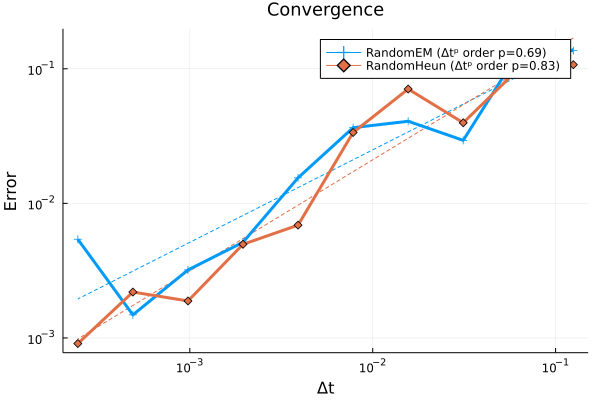
\includegraphics[scale=0.8]{img/plot_13.png}
\end{figure}

For a lower order convergence, below order $1$, we take the noise $\{Y_t\}_t$ to be the transport process defined by
$$
Y_t = \sin(t/Z)^{1/3},
$$
where $Z$ is a beta random variable $Z \sim B(\alpha, \beta)$. Notice $Z$ takes values strictly within $(0, 1)$ and, hence, $\sin(t/Z)$ can have arbitrarily high frequencies and, hence, go through the critic value $y = 0$ extremely often.

\textcolor{red}{(Need to remove the Heun method and do more tests)}.

\section*{Acknowledgments}


\begin{thebibliography}{25}
    \bibitem{Asai2016} Y. Asai, \emph{Numerical Methods for Random Ordinary Differential Equations and their Appli-
    cations in Biology and Medicine.} Dissertation, Institut für Mathematik, Goethe Universität Frankfurt am Main, 2016.

    \bibitem{CoddingtonLevinson1985} E. A. Coddington, N. Levinson, \emph{Theory of Ordinary Differential Equations,} New York: McGraw-Hill, 1987.

    \bibitem{GruneKloeden2001} L. Gr\"une, P.E. Kloeden, Higher order numerical schemes for affinely controlled nonlinear systems, \emph{Numer. Math.} 89 (2001), 669--690.

    \bibitem{HanKloeden2017} X. Han \& P. E. Kloeden (2017), \emph{Random Ordinary Differential Equations and Their Numerical Solution,} Probability Theory and Stochastic Modelling, vol. 85, Springer Singapore. \href{https://link.springer.com/book/10.1007/978-981-10-6265-0}{DOI: 10.1007/978-981-10-6265-0}.
\end{thebibliography}

\end{document}